\documentclass[a4paper, 10pt]{exam}
\usepackage[margin=1in]{geometry}

\usepackage[utf8]{inputenc}
\usepackage{amssymb, amsmath, graphicx, multicol}
\usepackage{pgf,tikz, graphicx}
\usepackage{mdframed}
\usepackage{mathrsfs}

\everymath{\displaystyle}
\printanswers
\newmdtheoremenv{proof}{Figure }

\begin{document}
\fbox{\textbf{Math 140 - HW 1.2}} 
\textbf{REGALARIO, Jeremiah Daniel A. | 2022-20670}
\begin{questions}
    \question Let $G$ be the geometry model with diagram
    \begin{center}
        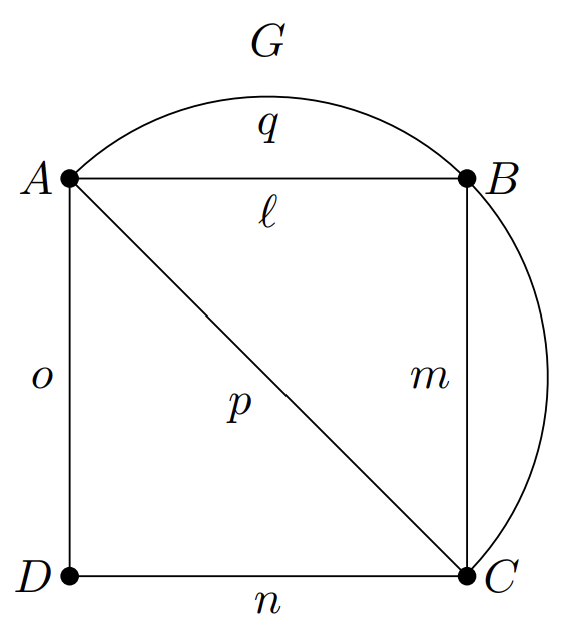
\includegraphics[width=0.3\textwidth]{1.2.png}
    \end{center}
Draw another diagram for $G$ where points are now visualized as segments/arcs and lines are now visualized as dots. Label each segment/arc $(A, B, C, D)$ and each dot $( \ell, m, n, o, p, q).$
    \begin{proof}
        \begin{center}
            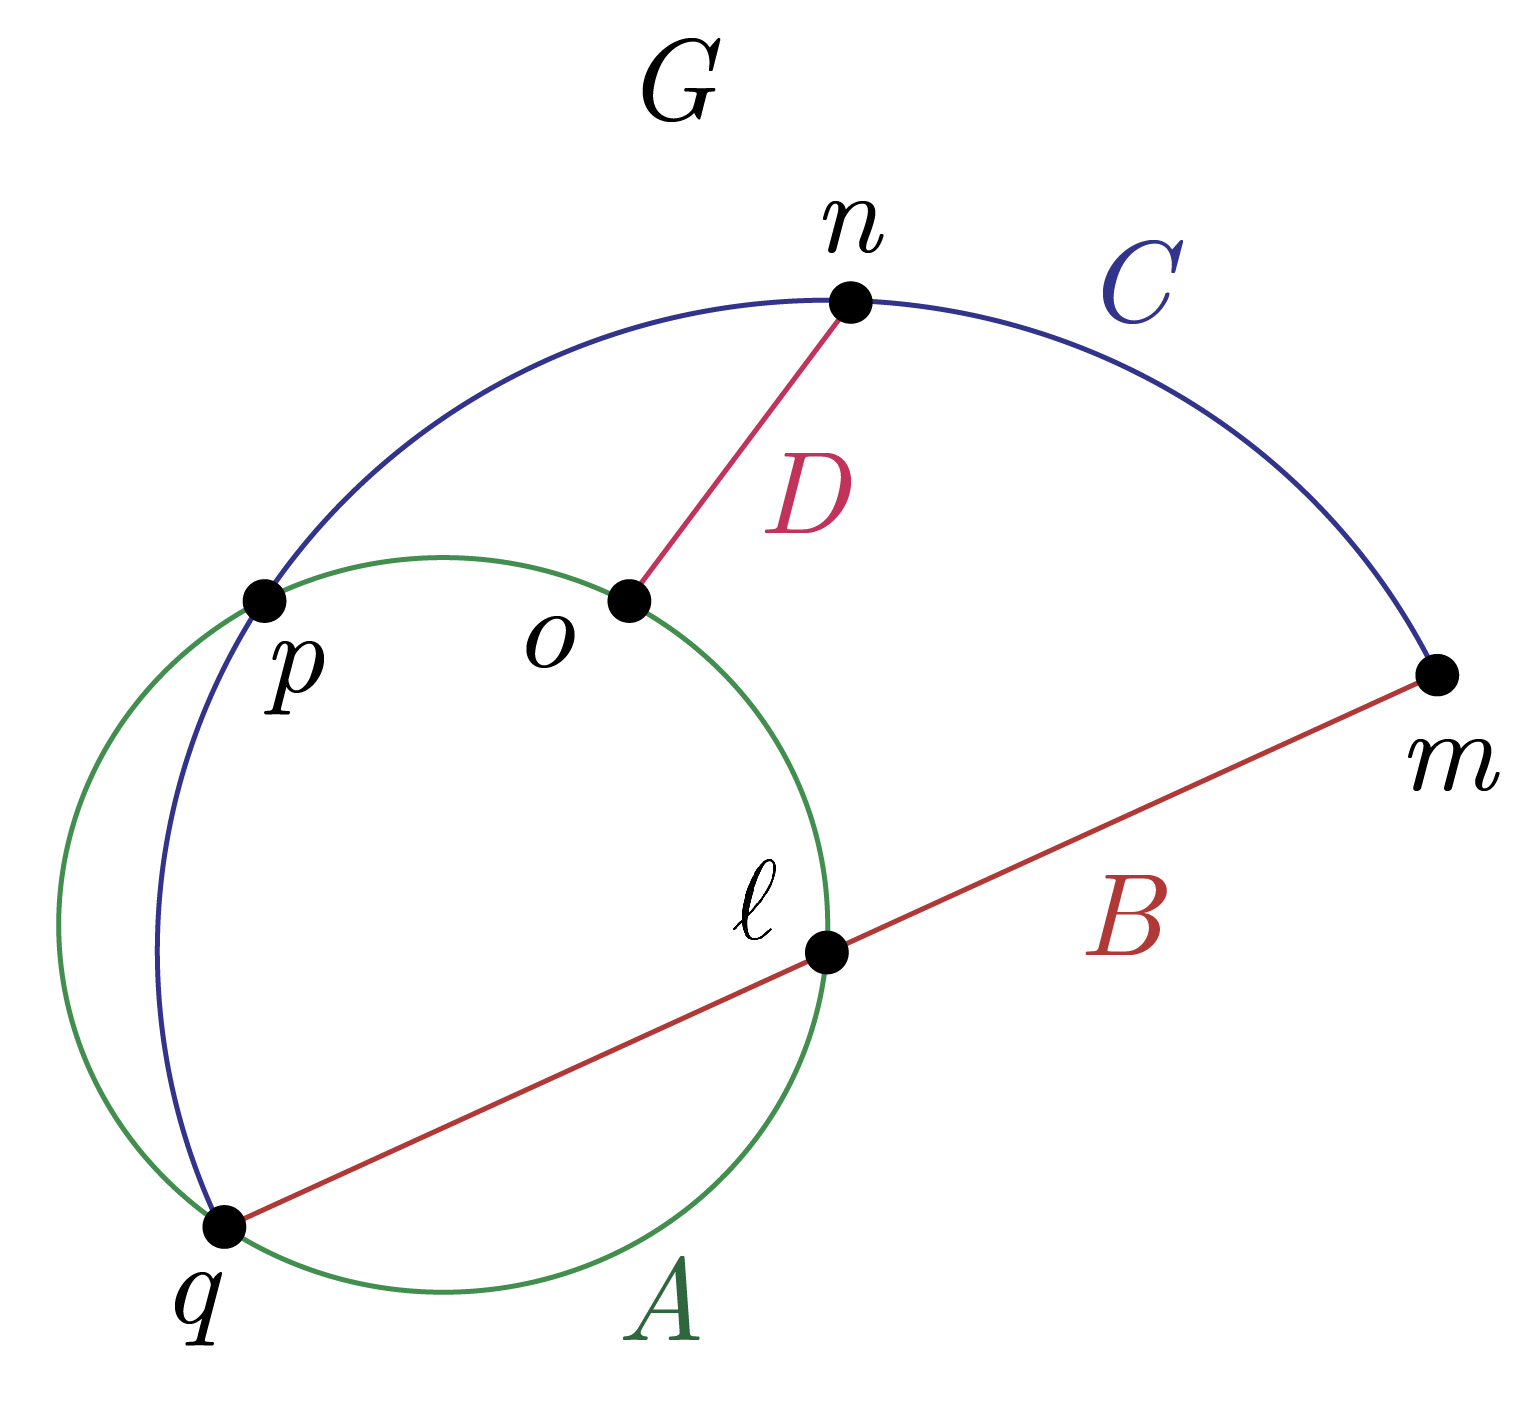
\includegraphics[width=0.4\textwidth]{2.1.png}
        \end{center}
        \\
    \end{proof}
    
\end{questions}

\end{document}
